\section{Business Model Canvas}
\label{BMC_Kapitel}
Die \ac{BMC} bezeichnet ein Geschäftsmodellkonzept. Osterwalder definiert ein Geschäftsmodell wie folgt:
\begin{quote}
Ein Geschäftsmodell beschreibt das Grundprinzip, nach dem eine Organisation Werte schafft, vermittelt und erfasst.
\end{quote}
Danach entwickelt er ein Muster, welches die Beschreibung eines Geschäftsmodells vereinfachen soll, indem es in neun Bausteine aufgeteilt wird. Unter einer Canvas versteht man hier eine übersichtliche Darstellung der wichtigsten Informationen, möglichst von dem Umfang einer Seite. So gliedert sich der Aufbau im Allgemeinen in zwei Hälften. Die rechte Seite der \ac{BMC} beschäftigt sich mit dem Wert der Organisation, wohingegen die linke Seite auf die Effizienz eingeht. Damit ist bereits auf einem Dokument ersichtlich, wie das Projekt effizient Werte vermitteln soll. Im Detail ist die \ac{BMC} in neun Bausteine aufgeteilt, welche in Abbildung \ref{BMC_Structure} dargestellt sind. Auf dieser Darstellung ist erkennbar, dass die rechte Seite auf den Wert für den Endnutzer abgestimmt ist, wohingegen sich die linke Seite eher auf die Verlagerung von Ressourcen spezialisiert, also die Effizienz, nach Osterwalder. 
\begin{figure}
	\begin{center}
		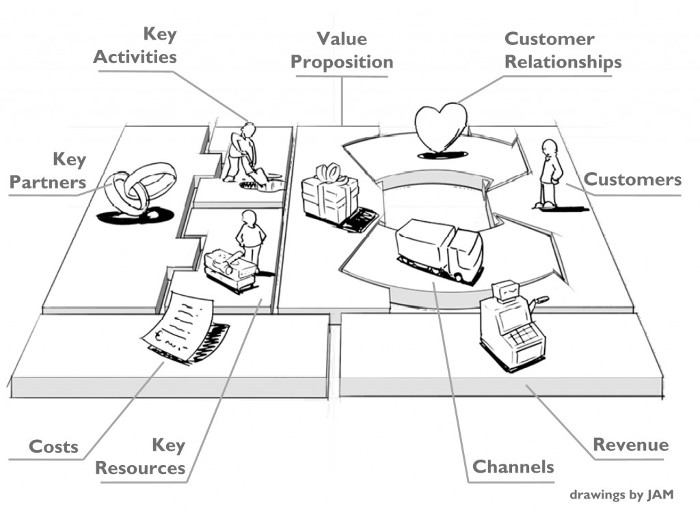
\includegraphics[width=\textwidth/2]{99_IMG/02_Grundlagen/bmcStructure.jpg}
		\caption[Struktureller Aufbau der \ac{BMC}]{Struktureller Aufbau der \ac{BMC}\cite{Sammer2018}}
		\label{BMC_Structure}
	\end{center}
\end{figure}
Die einzelnen Bausteine werden im Folgenden genauer erklärt:

\begin{itemize}
	\item \textbf{\ac{CS}}
	
	Die Kundensegmente beschreiben alle Kundengruppen des Unternehmens. Dabei ist es möglich, dass der Massenmarkt die Zielgruppe beschreibt. Zeilt ein Produkt allerdings nur auf eine bestimmte Art von Kunden mit ähnlichen Bedürfnissen und Wünschen ab, nennt sich das Nischenmarkt. Darüber hinaus können Kundengruppen segmentiert werden, da unterschiedliche Gruppen der gesamten Kundenmenge verschiedene Eigenschaften aufweisen, welche das Kauf- oder Nutzverhalten bestimmen kann. 
	
	\item \textbf{\ac{VP}}
	
	Die Mehrwerte, die das Produkt dem Endkunden bringt, werden hier als Wertangebote bezeichnet. Dabei kann grob in quantitative, also messbare, und qualitative Werte unterschieden werden. Genauer unterscheidet Osterwalder hier in die folgenden Kategorien: Neuheit, Leistung, Anpassung an Kundenwünsche, die Arbeit erleichternd, Design, Marke/Status, Preis, Kostenreduktion, Risikominderung, Verfügbarkeit.
	
	\item \textbf{\ac{CH}}
	
	Über welche Kanäle das Produkt dem Kunden vermittelt werden soll, wird in dieser Section dargestellt. Kanäle können in eigene und Partnerkanäle, sowie direkte und indirekte Kanäle unterschieden werden. Eigene direkte Kanaltypen stellen beispielsweise eine eigene Verkaufsabteilung oder direkter Verkauf über eine eigene Website dar. Dazu bietet eine eigene Filiale einen eigenen, aber indirekten Kanal dar, da der Verkauf über einen Mittelmann, die Filiale, stattfindet. Indirekte Partnerkanäle sind beispielsweise Partnerfilialen oder Großhändler. Ein Kanal verfügt nach Osterwalder über fünf Phasen. So muss zuerst die Aufmerksamkeit des Kunden erregt werden und diesem die Möglichkeit gegeben werden, das Produkt für sich zu bewerten. Darauf aufbauend soll der Kunde zum Kauf angeregt werden. Nach dem Kauf muss dem Nutzer der Wert des Produktes vermittelt werden und dieser muss auch weiterhin Unterstützung von Seiten des Unternehmens genießen können.
	
	\item \textbf{\ac{CR}}
	
	Die Art von Beziehungen, die ein Unternehmen mit den Kunden eingeht, wird unter \ac{CR} festgehalten. So kann ein Betrieb persönliche Unterstützung anbieten, was häufig am Point of Sale passiert. Geht diese Unterstützung tiefer ins Detail, kann dies auch Individuelle persönliche Unterstützung genannt werden. Darüber hinaus gibt es auch Selbstbedienung und Automatisierte Dienstleistungen als Arten von Kundenbeziehungen. Ersteres bezeichnet ein Unternehmen, welches keine direkte Kundeninteraktion führt, sondern den Kunden die Möglichkeit gibt, sich selbst zu bedienen. Diese Art der Kundenorientierung in Kombination mit automatisierten Prozessen wird Automatisierte Dienstleistung genannt. Des Weiteren kann ein Betrieb darauf setzen, die Kunden untereinander in einer Community zu vernetzen. Ein weiterer Weg, Beziehungen zu Kunden aufzubauen, kann es sein, diese zur Mitbeteiligung anzuregen, beispielsweise durch die Aufforderung zu Rezensionen.
	
	\item \textbf{\ac{Rdollar}}
	
	Die Einnahmequellen beschreiben die Umsatzart, die ein Unternehmen anstrebt. Die häufigsten Arten werden hier in folgende Bereiche unterteilt: Verkauf von Wirtschaftsgütern, Nutzungsgebühr, Mitgliedsgebühren, Verleih/Vermietung/Leasing, Lizenzen, Maklergebühren, Werbung. Außerdem wird in Festpreise und Variable Preise unterschieden. Ein Festpreis kann sich dabei durch bestimmte Produkteigenschaften, dem Kundensegment oder die Menge zusammensetzen. Allerdings ändert sich dieser nicht durch andere Einflüsse. Im Gegensatz dazu verändert sich ein variabler Preis beispielsweise durch Verhandlungen oder Auktionen. Dazu ist es möglich, dass der Echtzeitmarktwert, also das Zusammenspiel von Angebot und Nachfrage, oder das Ertragsmanagement, abhängig von Bestand und Kaufzeitpunkt, den Preis beeinflussen.
	
	
	\item \textbf{\ac{KR}}
	
	Unter diesem Punkt werden sämtliche Wirtschaftsgüter gelistet, welche für das Unternehmen benötigt werden. Dazu zählen beispielsweise physische Güter, wie Räumlichkeiten oder Maschinen. Außerdem kann eine Ressource auch menschlich sein. Dabei soll besonders auf die Kompetenzen der Kraft eingegangen werden. Auch finanzielle Güter können hier von Bedeutung sein.
	
	\item \textbf{\ac{KA}}
	
	Die Schlüsselaktivitäten umfassen alle Tätigkeiten, die benötigt werden, damit das Geschäftsmodell funktionieren kann. Unter Anderem können diese Aktivitäten die Produktion einer Ware, die Lösung eines Problemes oder die Vernetzung der Kunden beinhalten. 
	
	\item \textbf{\ac{KP}}
	
	Häufig werden Geschäftspartner benötigt, um das Geschäftskonzept umzusetzen, welche unter diesem Punkt aufgeführt werden. Der Autor unterteilt diese in drei Kategorien. Die erste Gruppe dient der Optimierung oder einem Mengenvorteil. Darunter versteht man beispielsweise die Zulieferung von Bauteilen oder das Auslagern von Infrastruktur. Eine weitere Partnerschaftskategorie dient der Minderung von Risiken und Unsicherheiten. Nicht selten kommt es vor, dass Konkurrenten zusammen an einer neuen Technologie forschen. Dabei kommt diese Art von Partnerschaft zustande. Die dritte Gruppe bildet die Akquise bestimmter Ressourcen und Aktivitäten. Hier werden etwa Kompetenzen oder Lizenzen anderer Unternehmen benötigt, um das eigene Produkt zu erstellen.
	
	\item \textbf{\ac{Cdollar}}
	
	Abschließend werden die Kosten aufgelistet, welche mit dem Geschäftsmodell verbunden sind. Dabei kann es unter Umständen sinnvoll sein, zwischen einer kostenorientierten oder wertorientierten Kostenstruktur zu unterscheiden. Kostenoerientiert bedeutet hier, dass der Fokus des Unternehmens darauf liegt, die Kosten zu senken. Im Gegensatz dazu liegt der Schwerpunkt eines wertorientierten Geschäftsmodells darin, dem Kunden maximalen Wert zu vermitteln. Der Autor nennt hier beispielhaft eine Billifluglinie als kostenorientiertes und ein Luxushotel als wertorientiertes Unternehmen. Meist liegt das Geschäftskonzept allerdings zwischen diesen Kategorien. Nichtsdestotrotz können die anfallenden Kosten auch andere Merkmale aufweisen. Hier kann etwa in Fix- oder variable Kosten unterschieden werden. Fixkosten ändern sich nicht, wohingegen variable Kosten etwa von der Menge der produzierten Waren abhängig ist. Außerdem sollten Mengen- und Verbundvorteile beachtet werden. Je mehr Waren ein Unternehmen produziert, desto geringer sind die anfallenden Kosten pro Produkt in der Regel. Dazu kann ein großer Betrieb davon profitieren, mehrere Produkte mit derselben Strategie zu vermarkten, was wiederum Kosten spart.
	
\end{itemize}

Diese Bausteine fassen das Geschäftsmodell prägnant zusammen, sodass mithilfe der Canvas die wichtigsten Details auf einen Blick erkennbar sind.
\cite{BusinessModelGeneration}